\documentclass[11pt,a4paper]{article}

% ---------------------------------------------------------------- packages
\usepackage[utf8]{inputenc}
\IfFileExists{lmodern.sty}{\usepackage[T1]{fontenc}\usepackage{lmodern}}{}
\usepackage[english]{babel}
\usepackage[a4paper,margin=2.5cm]{geometry}
\usepackage{microtype}
\usepackage{amsmath,amssymb}
\usepackage{graphicx}
\usepackage{booktabs}
\usepackage[font=small,labelfont=bf,skip=6pt]{caption}
\usepackage{subcaption}
\usepackage{xcolor}
\definecolor{linkblue}{HTML}{1F5FAD}
\usepackage[colorlinks=true,linkcolor=linkblue,citecolor=linkblue,urlcolor=linkblue]{hyperref}
\usepackage{titlesec}
\titleformat{\section}{\large\bfseries}{\thesection}{0.6em}{}
\titleformat{\subsection}{\normalsize\bfseries}{\thesubsection}{0.6em}{}
\titlespacing*{\section}{0pt}{14pt}{6pt}
\titlespacing*{\subsection}{0pt}{10pt}{4pt}
\setlength{\parskip}{3pt}
\usepackage{enumitem}

% ---------------------------------------------------------------- title
\title{\vspace{-1.2cm}\textbf{Can Machine Learning Predict If Your\\ TikTok Will Be a Hit or a Flop?}\\[4pt]
\large Predicting the Number of Likes of a Video from Its Metadata}
\author{Nathan Tessot\\[2pt]
\small CPES -- Data Science \& Cultural Sciences, Université PSL\\
\small Machine learning project\\[2pt]
\small \href{https://github.com/NathanTessot75/tiktok-analysis}{\texttt{github.com/NathanTessot75/tiktok-analysis}}}
\date{\small January 2026}

\begin{document}
\maketitle

% ---------------------------------------------------------------- abstract
\begin{abstract}
\noindent
This study aims to predict the number of likes a TikTok video will receive from
its characteristics and from metadata about its author. Using a dataset of
19,084 TikTok videos, I engineer 22 additional features and compare three
regression models: a linear regression, a LASSO regression and a neural network
(multilayer perceptron), with hyperparameters tuned by 5-fold cross-validation.
Models are evaluated with the root mean squared error (RMSE) on a held-out test
set. The neural network performs best, with a test RMSE of 44,533 likes and a
test $R^2$ of 0.89, against about 50,000 likes and $R^2 \approx 0.86$ for the
two linear models. Train and test errors are almost identical for all three
models, which points to bias rather than overfitting as their main limitation.
\end{abstract}

% ---------------------------------------------------------------- 1
\section{Introduction}

Predicting the number of likes a TikTok video will receive is a valuable task
in social media analytics: it can guide content creation, advertising
strategies and platform optimization. The goal of this project is to predict the
number of likes of a video from its characteristics (duration, views, shares,
comments, downloads, transcription) and from the status of its author (verified
account, banned or under review).

Since the target is a continuous count, this is a regression problem. I compare
a simple linear baseline, a regularized linear model and a non-linear model, to
see how much flexibility the task requires.

% ---------------------------------------------------------------- 2
\section{Data}

The data is a public dataset of TikTok videos, available on Kaggle, in which
each video is labelled as stating a \emph{claim} or an \emph{opinion}. It
contains 19,382 videos; removing rows with missing values leaves
$N = 19{,}084$ videos. Each video is described by 12 variables: claim status,
duration, transcription text, verified status and ban status of the author, and
the counts of views, likes, shares, downloads and comments.

The number of likes is extremely skewed (Figure~\ref{fig:likes}): the median
video receives about 3,400 likes, while the mean is about 84,000 and the
maximum exceeds 650,000. The distribution is clearly bimodal, which largely
reflects the claim status: the median ``claim'' video receives about 124,000
likes, against about 800 for ``opinion'' videos.

\begin{figure}[t]
  \centering
  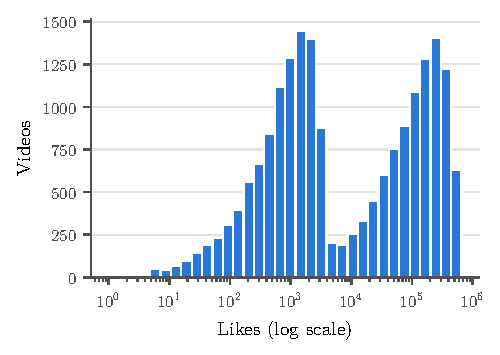
\includegraphics[width=0.46\linewidth]{figures/fig1_likes_distribution.pdf}
  \caption{Distribution of the number of likes ($N = 19{,}084$ videos, log scale).}
  \label{fig:likes}
\end{figure}

% ---------------------------------------------------------------- 3
\section{Method}

\paragraph{Feature engineering.} I created 22 new variables, for a total of 27
predictors: engagement ratios (shares, comments and downloads per view; views
per comment and per download; comments and shares per download); log
transformations of the views, comments, shares and downloads, and a total
engagement volume; duration-based rates (views, comments, shares and
interactions per second); encoded categorical variables (verified account, ban
status, claim status); and simple text features from the transcription
(length, number of words, average word length).

\paragraph{Protocol.} All predictors are standardized. The data is split into a
training set (75\%, 14,313 videos) and a test set (25\%, 4,771 videos). Three
models are trained:
\begin{itemize}[itemsep=1pt, topsep=2pt]
  \item a \textbf{linear regression}, as a baseline;
  \item a \textbf{LASSO regression}, whose regularization strength $\alpha$ is
  tuned by 5-fold cross-validation over seven values from 1 to $10^6$
  (35 fits);
  \item a \textbf{neural network} (multilayer perceptron with early stopping),
  whose architecture, activation function, solver, learning rate and batch size
  are tuned by 5-fold cross-validation over 120 combinations (600 fits;
  Table~\ref{tab:hyper}).
\end{itemize}

\paragraph{Metric.} Since I want to avoid large prediction errors, models are
compared with the root mean squared error (RMSE), which penalizes large
deviations more heavily. I also report the coefficient of determination $R^2$
on the test set.

% ---------------------------------------------------------------- 4
\section{Results}

Table~\ref{tab:results} summarizes the performance of the three models, and
Figure~\ref{fig:pred} compares their predictions with the actual number of
likes.

\begin{table}[h]
  \centering
  \small
  \begin{tabular}{lrrr}
    \toprule
    Model & Train RMSE & Test RMSE & Test $R^2$ \\
    \midrule
    Linear regression & 49,436 & 49,927 & 0.864 \\
    LASSO regression ($\alpha = 1000$) & 49,882 & 50,410 & 0.861 \\
    \textbf{Neural network} & \textbf{44,611} & \textbf{44,533} & \textbf{0.891} \\
    \bottomrule
  \end{tabular}
  \caption{Performance of the three models (RMSE in number of likes).}
  \label{tab:results}
\end{table}

\begin{figure}[h]
  \centering
  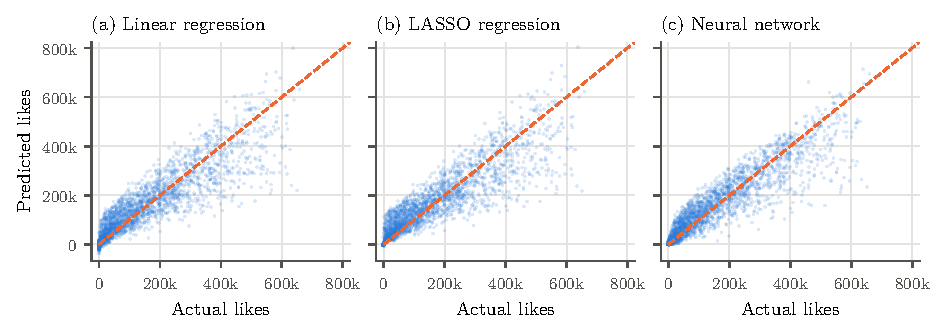
\includegraphics[width=\linewidth]{figures/fig2_predicted_vs_actual.pdf}
  \caption{Predicted versus actual number of likes on the test set. The dashed
  line marks perfect predictions.}
  \label{fig:pred}
\end{figure}

\subsection{Linear regression}

The linear regression reaches an RMSE of 49,436 on the training set and 49,927
on the test set (Figure~\ref{fig:pred}a). The small gap between the two
suggests low variance, but the level of the error indicates that the model
suffers from bias: a linear combination of the features cannot capture the
whole relationship. The model also handles the many videos with few likes
poorly: about a fifth of its test predictions are negative, which is
impossible for a count.

\subsection{LASSO regression}

Cross-validation selects $\alpha = 1000$. The LASSO reaches an RMSE of 49,882
on the training set and 50,410 on the test set (Figure~\ref{fig:pred}b), very
close to the unregularized model. Since the linear regression did not overfit,
regularization brings no gain here: the problem is bias, not variance.

\subsection{Neural network}

The selected network has two hidden layers of 8 and 4 units with ReLU
activations, trained with Adam (learning rate 0.01, batch size 32;
Table~\ref{tab:hyper}). It reaches an RMSE of 44,611 on the training set and
44,533 on the test set (Figure~\ref{fig:pred}c), about 11\% lower than the
linear models. Its predictions follow the diagonal more closely and are never
negative: for videos with fewer than 10,000 likes, its mean absolute error is
about 1,400 likes, against 4,800 for the linear regression.

The learning curve (Figure~\ref{fig:curve}) shows that the network needs about
250 iterations to stabilize. Train and test errors stay very close throughout
training and plateau together around 43,500 likes: the model does not overfit,
and its remaining error is mostly bias.

\begin{figure}[h]
  \centering
  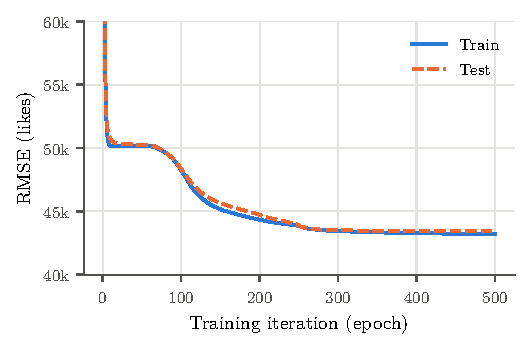
\includegraphics[width=0.58\linewidth]{figures/fig3_learning_curve.pdf}
  \caption{Train and test RMSE of the selected neural network across training
  iterations.}
  \label{fig:curve}
\end{figure}

% ---------------------------------------------------------------- 5
\section{Conclusion}

The neural network is the best model, with a test RMSE of 44,533 likes and a
test $R^2$ of 0.89. Its error is about a third of the standard deviation of
likes (about 135,000 on the test set), and the close match between train and
test errors shows that it generalizes well. User metadata and video
characteristics therefore carry a strong signal about the number of likes.

These results come with two caveats. First, the RMSE is dominated by the most
popular videos: an average error of 44,000 likes is small for a video with
500,000 likes but very large for the typical video, which receives about 3,400.
Modelling the logarithm of likes, or reporting a relative error, would give a
fairer picture across the whole distribution. Second, the strongest predictors
(views, shares, comments) are measured at the same time as the likes. The
models therefore explain the likes of a video that has already been published
rather than predict, before publication, whether it will be a hit. Predicting
success ahead of time would require features available at upload, such as the
content of the video, its author's history or the publication time.

% ---------------------------------------------------------------- appendix
\appendix
\section{Neural network hyperparameters}

\begin{table}[h]
  \centering
  \small
  \begin{tabular}{lll}
    \toprule
    Hyperparameter & Tested values & Selected value \\
    \midrule
    Hidden layer sizes & (1), (2), (2, 2), (4, 2), (8, 4) & (8, 4) \\
    Activation function & ReLU, tanh, logistic & ReLU \\
    Solver & Adam, SGD & Adam \\
    Initial learning rate & 0.001, 0.01 & 0.01 \\
    Batch size & 32, 64 & 32 \\
    \bottomrule
  \end{tabular}
  \caption{Hyperparameters tested in 5-fold cross-validation (120 combinations,
  600 fits). Early stopping is used in every configuration.}
  \label{tab:hyper}
\end{table}

\end{document}
